\subsection{Swap}
It would also be smart if we could swap out modules in the configuration with free modules, or two modules within a configuration that is capable of doing each others active work.

For this we describe two sets, $Swap_{extern}$ and $Swap_{intern}$. These sets contain all pairs of modules which we can swap with each other. A graph showing each of the swap rules can be seen respectively in \cref{fig:swap_ext} and \cref{fig:swap_int}.

\[Swap_{extern} = \{(m, m') | m \in CM \land m' \in FM \land m.aW \subseteq m'.mW \}\]

\[Swap_{intern} = \{(m, m') | m, m' \in CM \land m.aW \subseteq m'.mW \land m'.aW \subseteq m.mW \}\]

\begin{figure}[h]
\centering
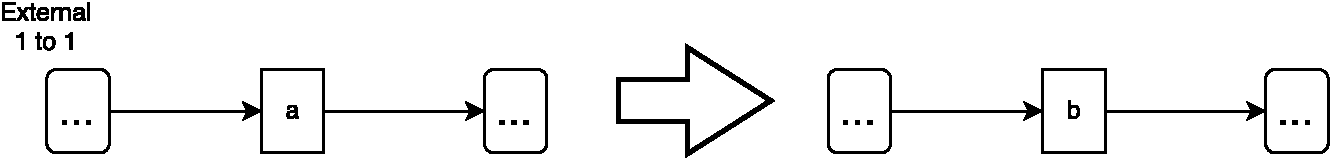
\includegraphics[width=0.8\textwidth]{swap_ext.pdf}
\caption{External swap rule. Here $a$ denotes the first element in a pair from $Swap_{extern}$ and $b$ denotes the second element}
\label{fig:swap_ext}
\end{figure}

\begin{figure}[h]
\centering
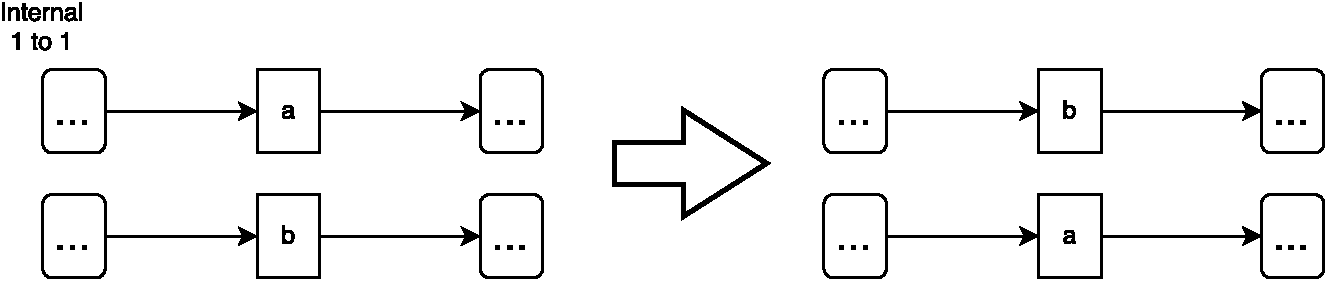
\includegraphics[width=0.8\textwidth]{swap_int.pdf}
\caption{Internal swap rule. Here $a$ denotes the first element in a pair from $Swap_{intern}$ and $b$ denotes the second element}
\label{fig:swap_int}
\end{figure}

For the extern case in \cref{fig:swap_ext} we simply swap out the first element of a pair in $Swap_{extern}$ with the second element of the pair. Assigning the $up$, $right$, $down$, $left$ and $aW$ attributes of the second element equal to that of the first. We also remove the first element from the line it was in and insert the second in its stead, with the same total ordering.

We do something similar for the intern case in \cref{fig:swap_ext}. Here we instead of removing one of the two element in the pair, we assign the $up$, $right$, $down$, $left$ and $aW$ attributes of both elements to that of the other, and swap them in their respective lines.

We also need to describe that not all available modules need to be a part of our factory configuration. There may exist free modules, which are not used, but may aid in the search for a higher throughput. First we describe the set of all modules used by a configuration, denoted $CM$:

%\[CM = \{m \in \gamma | \gamma \in \Gamma \}\]
%The set of free modules $FM$ is then given by:
%\[FM = M \setminus CM \]
